\documentclass[tikz,border=10pt]{standalone}
\usepackage[utf8]{inputenc}
\usepackage[T1]{fontenc}
\usepackage{lmodern}
\usepackage{tikz}
\usetikzlibrary{shapes.geometric, arrows.meta, positioning, calc, backgrounds, fit}

\begin{document}
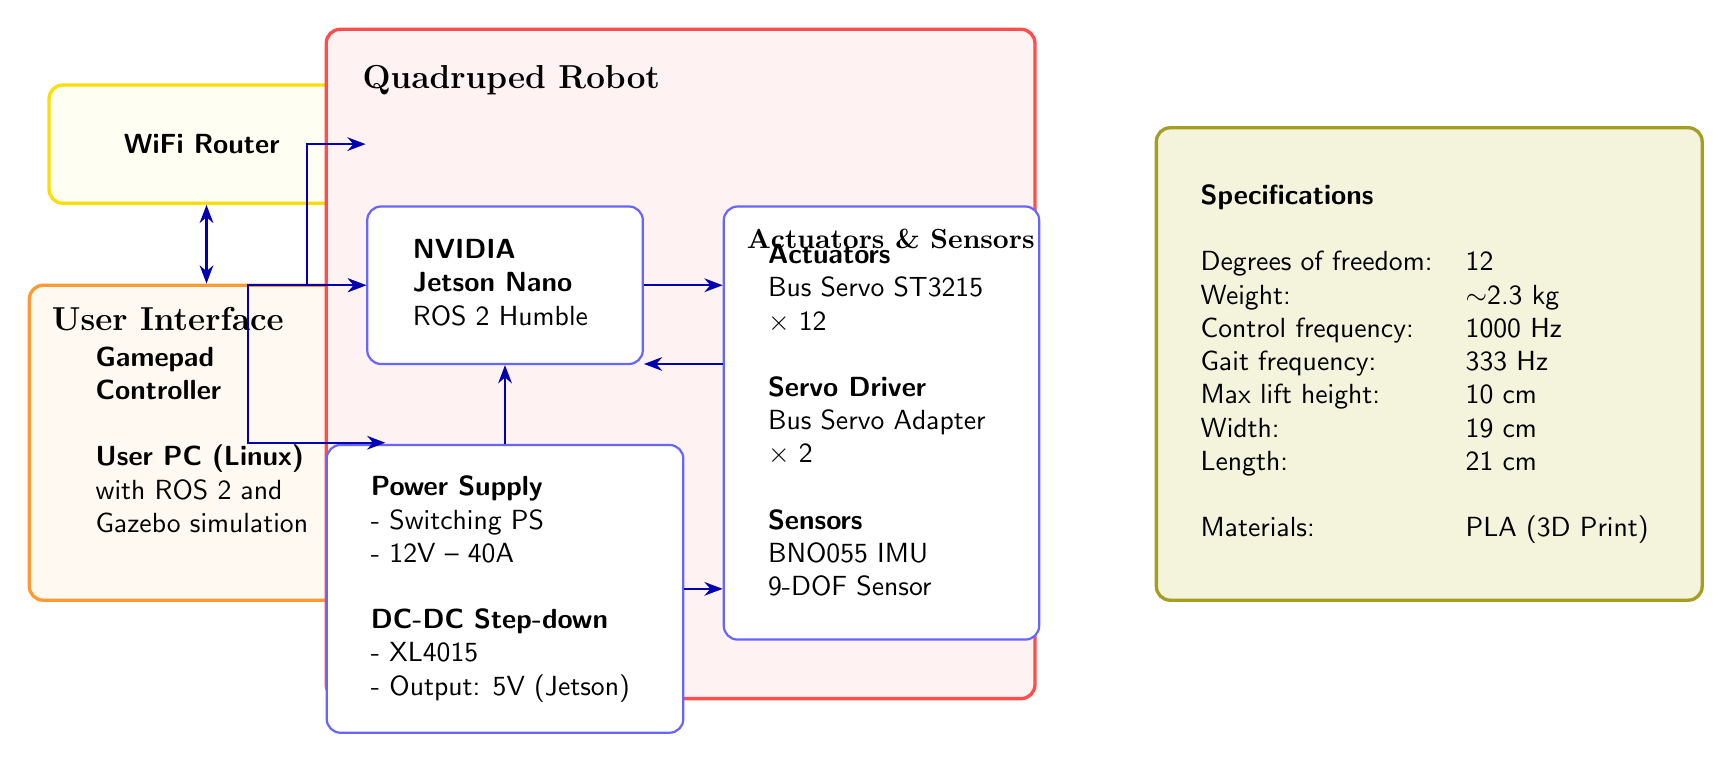
\begin{tikzpicture}[
    font=\sffamily,
    >=Stealth,
    thick,
    box/.style={draw, rounded corners=5pt, inner sep=10pt, align=left},
    mainbox/.style={box, very thick},
    title/.style={font=\bfseries\large, text=black},
    subtitle/.style={font=\bfseries, text=black},
    item/.style={font=\small},
    arrow/.style={->, thick, draw=blue!70!black}
]

% 1. User Interface Group (Left)
\node[mainbox, draw=yellow!80!orange, fill=yellow!5, minimum width=4cm, minimum height=1.5cm] (Router) {
    \textbf{WiFi Router}
};

\node[mainbox, draw=orange!80, fill=orange!5, minimum width=4.5cm, minimum height=4cm, below=1cm of Router] (UserInterface) {
    \begin{tabular}{l}
        \textbf{Gamepad} \\
        \textbf{Controller} \\
        \\
        \textbf{User PC (Linux)} \\
        with ROS~2 and \\
        Gazebo simulation
    \end{tabular}
};
\node[title, anchor=north west, xshift=5pt, yshift=-5pt] at (UserInterface.north west) {User Interface};

% 2. Robot Group (Middle)
\node[mainbox, draw=red!70, fill=red!5, minimum width=9cm, minimum height=8.5cm, right=1.5cm of UserInterface.center, yshift=1cm] (Robot) {};
\node[title, anchor=north west, xshift=10pt, yshift=-10pt] at (Robot.north west) {Quadruped Robot};

% Brain
\node[box, draw=blue!60, fill=white, minimum width=3.5cm, minimum height=2cm, anchor=west, xshift=15pt, yshift=1cm] (Brain) at (Robot.west) {
    \begin{tabular}{l}
        \textbf{NVIDIA} \\
        \textbf{Jetson Nano} \\
        ROS~2 Humble
    \end{tabular}
};

% Power
\node[box, draw=blue!60, fill=white, minimum width=3.5cm, minimum height=2.5cm, below=1cm of Brain] (Power) {
    \begin{tabular}{l}
        \textbf{Power Supply} \\
        - Switching PS \\
        - 12V -- 40A \\
        \\
        \textbf{DC-DC Step-down} \\
        - XL4015 \\
        - Output: 5V (Jetson)
    \end{tabular}
};

% Actuators & Sensors
\node[box, draw=blue!60, fill=white, minimum width=4cm, minimum height=5.5cm, right=1cm of Brain.north east, anchor=north west] (Actuators) {
    \begin{tabular}{l}
        \textbf{Actuators} \\
        Bus Servo ST3215 \\
        $\times$ 12 \\
        \\
        \textbf{Servo Driver} \\
        Bus Servo Adapter \\
        $\times$ 2 \\
        \\
        \textbf{Sensors} \\
        BNO055 IMU \\
        9-DOF Sensor
    \end{tabular}
};
\node[subtitle, anchor=north west, xshift=5pt, yshift=-5pt] at (Actuators.north west) {Actuators \& Sensors};

% 3. Specifications (Right)
\node[mainbox, draw=olive!80, fill=olive!10, minimum width=4cm, minimum height=6cm, right=1.5cm of Robot] (Specs) {
    \begin{tabular}{ll}
        \multicolumn{2}{l}{\textbf{Specifications}} \\
        \\
        Degrees of freedom: & 12 \\
        Weight: & $\sim$2.3 kg \\
        Control frequency: & 1000 Hz \\
        Gait frequency: & 333 Hz \\
        Max lift height: & 10 cm \\
        Width: & 19 cm \\
        Length: & 21 cm \\
        \\
        Materials: & PLA (3D Print)
    \end{tabular}
};

% Arrows
\draw[<->, thick, draw=blue!70!black] (UserInterface.north) -- (Router.south);
\draw[<->, thick, draw=blue!70!black] (Router.east) -| ([xshift=-0.75cm]Brain.west) -- (Brain.west);
\draw[<->, thick, draw=blue!70!black] (UserInterface.east) -- ([xshift=-1.5cm]Brain.west |- UserInterface.east) |- (Brain.west);

\draw[->, thick, draw=blue!70!black] (Brain.east) -- (Actuators.west |- Brain.east);
\draw[<-, thick, draw=blue!70!black] ([yshift=-1cm]Brain.east) -- ([yshift=-1cm]Actuators.west |- Brain.east);

\draw[->, thick, draw=blue!70!black] (Power.east) -- (Actuators.west |- Power.east);
\draw[->, thick, draw=blue!70!black] (Power.north) -- (Brain.south);

\end{tikzpicture}
\end{document}
